\documentclass[conference]{IEEEtran}

\usepackage{IEEEpreamble}
\usepackage{booktabs}

%\newcommand{\purpose}[1]{\textsc{\textbf{#1}}}
\newcommand{\purpose}[1]{}

\begin{document}
%
% paper title
% can use linebreaks \\ within to get better formatting as desired

\title{Commit Bubbles: A Fragment-based Approach to Software Configuration Management}

%\title{Flossy History Revision Editing for Version Control Commits}

% \title{Version control interventions: helping developers avoid cognitive breakdowns for more effective change management}

\author{\IEEEauthorblockN{Titus Barik,
Kevin Lubick,
Emerson Murphy-Hill}
\IEEEauthorblockA{North Carolina State University, USA\\
\{tbarik,kjlubick\}@ncsu.edu, emerson@csc.ncsu.edu}
}

% use for special paper notices
%\IEEEspecialpapernotice{(Invited Paper)}

% make the title area
\maketitle

\begin{abstract}
%\boldmath
When working with version control systems, developers are expected to follow a set of best practices, 
such as constructing systematic commit histories. 
These systematic commit histories should show well-defined steps with logical forward progress. 
Yet, the process by which developers write source code is frequently evolutionary, or as-needed, rather than systematic. 
We argue that the as-needed strategy that developers use to write code is incompatible with the strategy
that developers would need to use in order to generate systematic histories, yielding non-ideal commit histories. 
Our vision is a development model that reconciles as-needed activities with systematic commit activities. 
Our proposed tool, Commit Bubbles, operationalizes this vision by extending the working set metaphor used by 
Code Bubbles to support commit activities within the same environment that developers use to edit code. 
We hypothesize that this approach will enable developers to fluidly construct better commit histories using 
an interaction modality that is already familiar to developers.
\end{abstract}

% no keywords

% For peer review papers, you can put extra information on the cover
% page as needed:
% \ifCLASSOPTIONpeerreview
% \begin{center} \bfseries EDICS Category: 3-BBND \end{center}
% \fi
%
% For peerreview papers, this IEEEtran command inserts a page break and
% creates the second title. It will be ignored for other modes.
\IEEEpeerreviewmaketitle

\section{Motivation}

\purpose{Best practices for version control commit messages.} 
There are many best practices when adding commits to version control commit histories. 
For the commit itself, these best practices include using a descriptive commit message, 
avoiding indiscriminate commits, and making each commit a ``logical unit'' --- such that 
each commit has a singular purpose.\footnote{\url{http://homes.cs.washington.edu/~mernst/advice/version-control.html}} 
Extending this idea, the resulting \emph{published} commit histories should, in some sense, be \emph{systematic}, 
in that the history shows well-defined steps, each with logical forward progress, telling a cohesive narrative without 
broken or suboptimal steps~\cite{Loeliger2012}.

\purpose{Coding activities use a different model than what VCS requires.} 
Yet the way in which developers write and edit source code is frequently done in less of a \emph{systematic} way,
 and more of an evolutionary, or \emph{as-needed}, way~\cite{Perry1989,Littman1987}. 
 Littman, noting the dichotomy between systematic version histories and as-needed coding processes, elaborates, 
 ``trying to force this evolutionary process [coding] into neat, distinct, and independent phases [commits] only serves
  to obscure the reality of software development''~\cite{Littman1987}.

\purpose{Problem is that strategies are incompatible.} 
The fundamental problem is that the as-needed strategy that developers frequently use to write code is incompatible with 
the systematic strategy that developers would need to use in order to generate their published commit histories. 
As evidence, Murphy-Hill and colleagues found that refactoring operations are performed frequently, and that programmers 
frequently interleave refactoring with other types of programming activity. Similarly, Negara and colleagues found that 
46\% of refactored program entities are interspersed with other changes, and that 40\% of test fixes involve changes to the tests themselves~\cite{Negara2012}. In version control histories, these as-needed edits manifest themselves as \emph{tangled} commits, that is, commits that contain two or more logical units of changes~\cite{Kirinuki2014}, and as incomplete or incorrect commit messages, which fail to capture the full description of the change~\cite{Buse2010}. Both of these issues are obstacles to supporting downstream change management tasks, such as merging commits between branches, and conducting effective code reviews~\cite{Kirinuki2014}.

Our insight is that commit histories need not be immutable. 
In modern version control systems, history revision operations, such as \emph{rebase}, 
offer a mechanism by which a developer can take imperfect, as-needed commit histories and translate them to 
desired systematic commits.
\footnote{Robertson calls this ``sausage making'' --- ``The process of developing software, 
similar to the process of making sausage, is a messy messy business \ldots If you hide the sausage making, 
you can create a beautiful looking history where each step looks as delicious as the end-product.'' 
(\url{http://sethrobertson.github.io/GitBestPractices/})} 
In this paper, we argue that the primary barrier to performing effective history revision is not simply 
a problem of technical feasibility, but rather, that current tool approaches inadequately align their tool 
functionality with developer workflows~\cite{PerezDeRosso2013}.

First, revision activities, if they occur at all, are typically performed as a distinct activity from coding~\cite{Perry1989}. 
This context switch makes it difficult to remember all of the change activities related to a particular commit, 
since human memory is failure-prone, especially after interruption.~\cite{Parnin2012}. 
Second, history revision as supported in tools today takes the perspective that histories are typically correct and that 
revision is an exceptional situation. However, exceptions are normal in work processes, and tools should support handling 
exceptional situations as routine~\cite{Ackerman2000}.

Our vision is a development model that reconciles as-needed coding activities with systematic commit activities. 
We operationalize this model by adding commit support to \emph{Code Bubbles}, a metaphor and tool that allows developers 
to reason in terms of fragments and working sets, and allows for fluid rearrangement and manipulation of these working sets~\cite{Bragdon2010a}.
We postulate that developers can benefit from reasoning about commit activities in the same way. 
Our proposed extension, \emph{Commit Bubbles}, supports developers by a) blending coding and commit activities as a 
unified activity, and b) treating history revision as a routine, rather than exceptional process. 
We hypothesize that our approach will enable developers to construct better commit histories with less cognitive effort, 
while integrating with their existing coding workflow in an interaction modality that is already familiar to developers.

\section{TACO -- Tool Assisted Commit Operations}
\begin{figure}
\centering
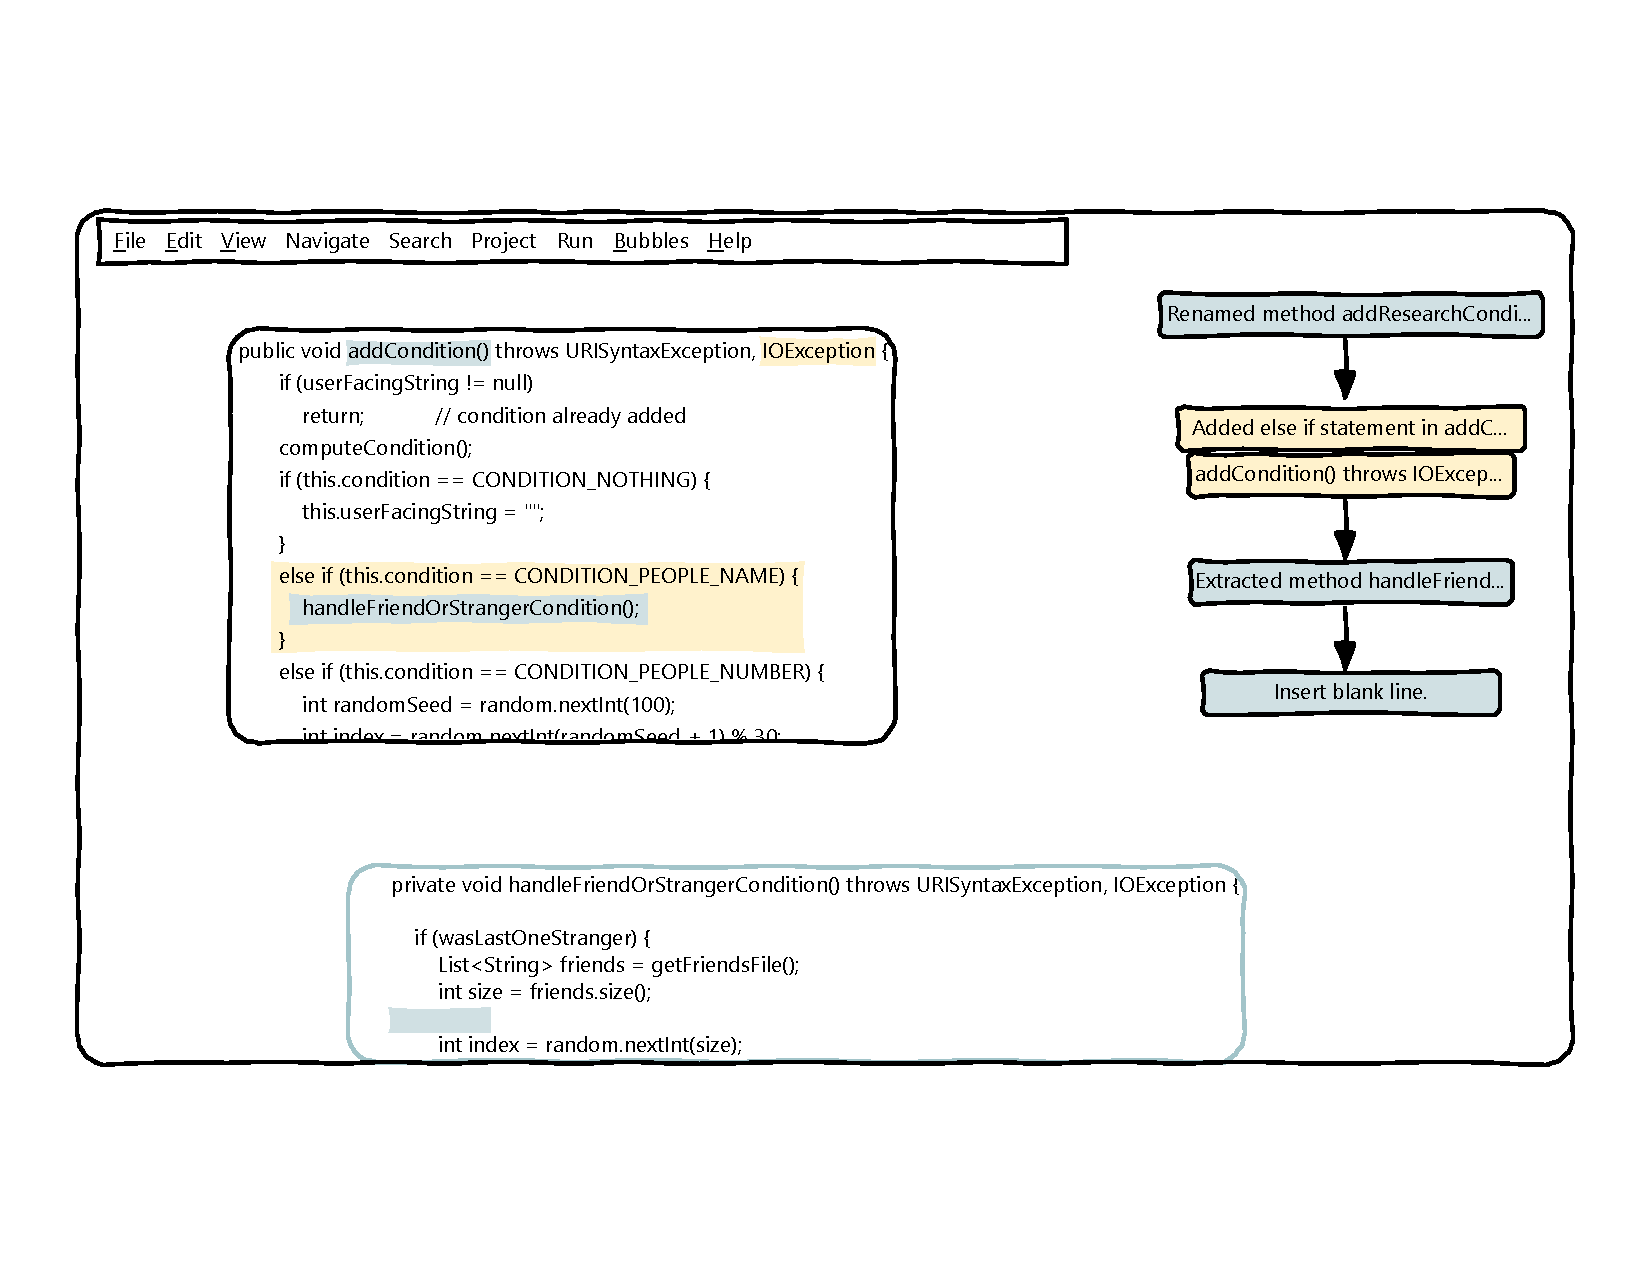
\includegraphics[width=3.5in]{commit-bubbles}
\caption{A mockup of TACO, showing the commit bubbles (A), the mouseovers (B),
and the change notifications (C)}
\label{fig:eclipse}
\end{figure}
\subsection{Commit Bubbles}
As a developer writes code, the IDE detects changes to the AST and autogenerates small commits
that conform to the one commit = one change rule.
These autocommits are placed in bubbles ordered chronologically from the top down.
The colors of the bubble indicate the type of commit; in this example, green commits mean nothing
semantic happened (e.g. refactoring) and yellow commits indicate logic changes.
These autogenerated messages are meant to help the developer remember roughly what happened and
easily deal with trivial commits and they are free to change the messages to suit their needs.

At any time, the developer may drag these commit bubbles around to reorder the history of the code,
combine two or more bubbles into one bigger feature set, do a \textit{soft delete}
or a \textit{hard delete} of one of the bubbles.
If a developer soft deletes a commit bubble, it won't go into the published history, but will still be a temporary artifact of their code base.
Suppose Jim, our example developer from earlier, wishes to insert some log statements or perform
some other test changes while debugging.  
Soft deleting allows him to prune the public history of these debugging artifacts, while still maintaining them in his code.
Hard deletions remove both the commit bubble and the corresponding code segments from the code base and the history. 

Developers clear these commit bubbles out when they press the ``commit'' button, saving them in the VCS.  
For a short while afterwards, they may undo this commit, repopulating the commit bubbles, allowing them to change their minds about what was saved to the public history.
\subsection{Synchronized mouseovers}
As each commit bubble is made, a small colored overlay appears next to the lines with the corresponding change.
These overlays offer developers a visual cue as to how much code has been changed since they 
committed their last set of commit bubbles.
Mousing over these overlays highlights the appropriate code bubble or bubbles,
reminding developers what changes occurred.

There is a temporal aspect of these overlays as well.
If more than one commit bubble impacts a line of code, the overlays stack
themselves left to right, helping keep the recent history in the mind of 
the developer.

\subsection{External Change notifications}
Software developed by groups of people can be prone to the same piece of code
being modified by multiple people at the same time.
TACO watches the public history of the code base and warns developers
of potential conflicts as they type.  
This way, merge conflicts can be dealt with earlier, rather than later.
Additionally, if the development team is collaborating using TACO, they
may also be notified if refactorings like file renames may impact their work, again, allowing earlier responses and easier resolutions.

\section{Example User Experience}
Software Developer Anthony is investigating a bug report about the Eclipse JDT crashing with a NullPointerException
He follows the stack trace to a method shouldIgnoreOptionalProblems, a method he hasn't worked with before.
The stacktrace doesn't indicate which variable was null, so Anthony decides to improve readability and debugability 
to the code by extracting the broken logic to a self-explaining method isParentOf.
Anthony adds in a few debug print statements (resulting in the code in Figure \ref{fig:eclipse}) and then writes a test replicating 
the steps in the bug report.
The print statements indicate that a null fileName is the root cause, so Anthony adds in an additional check,
leaving his commit bubbles looking like:
\begin{figure}[h]
\centering
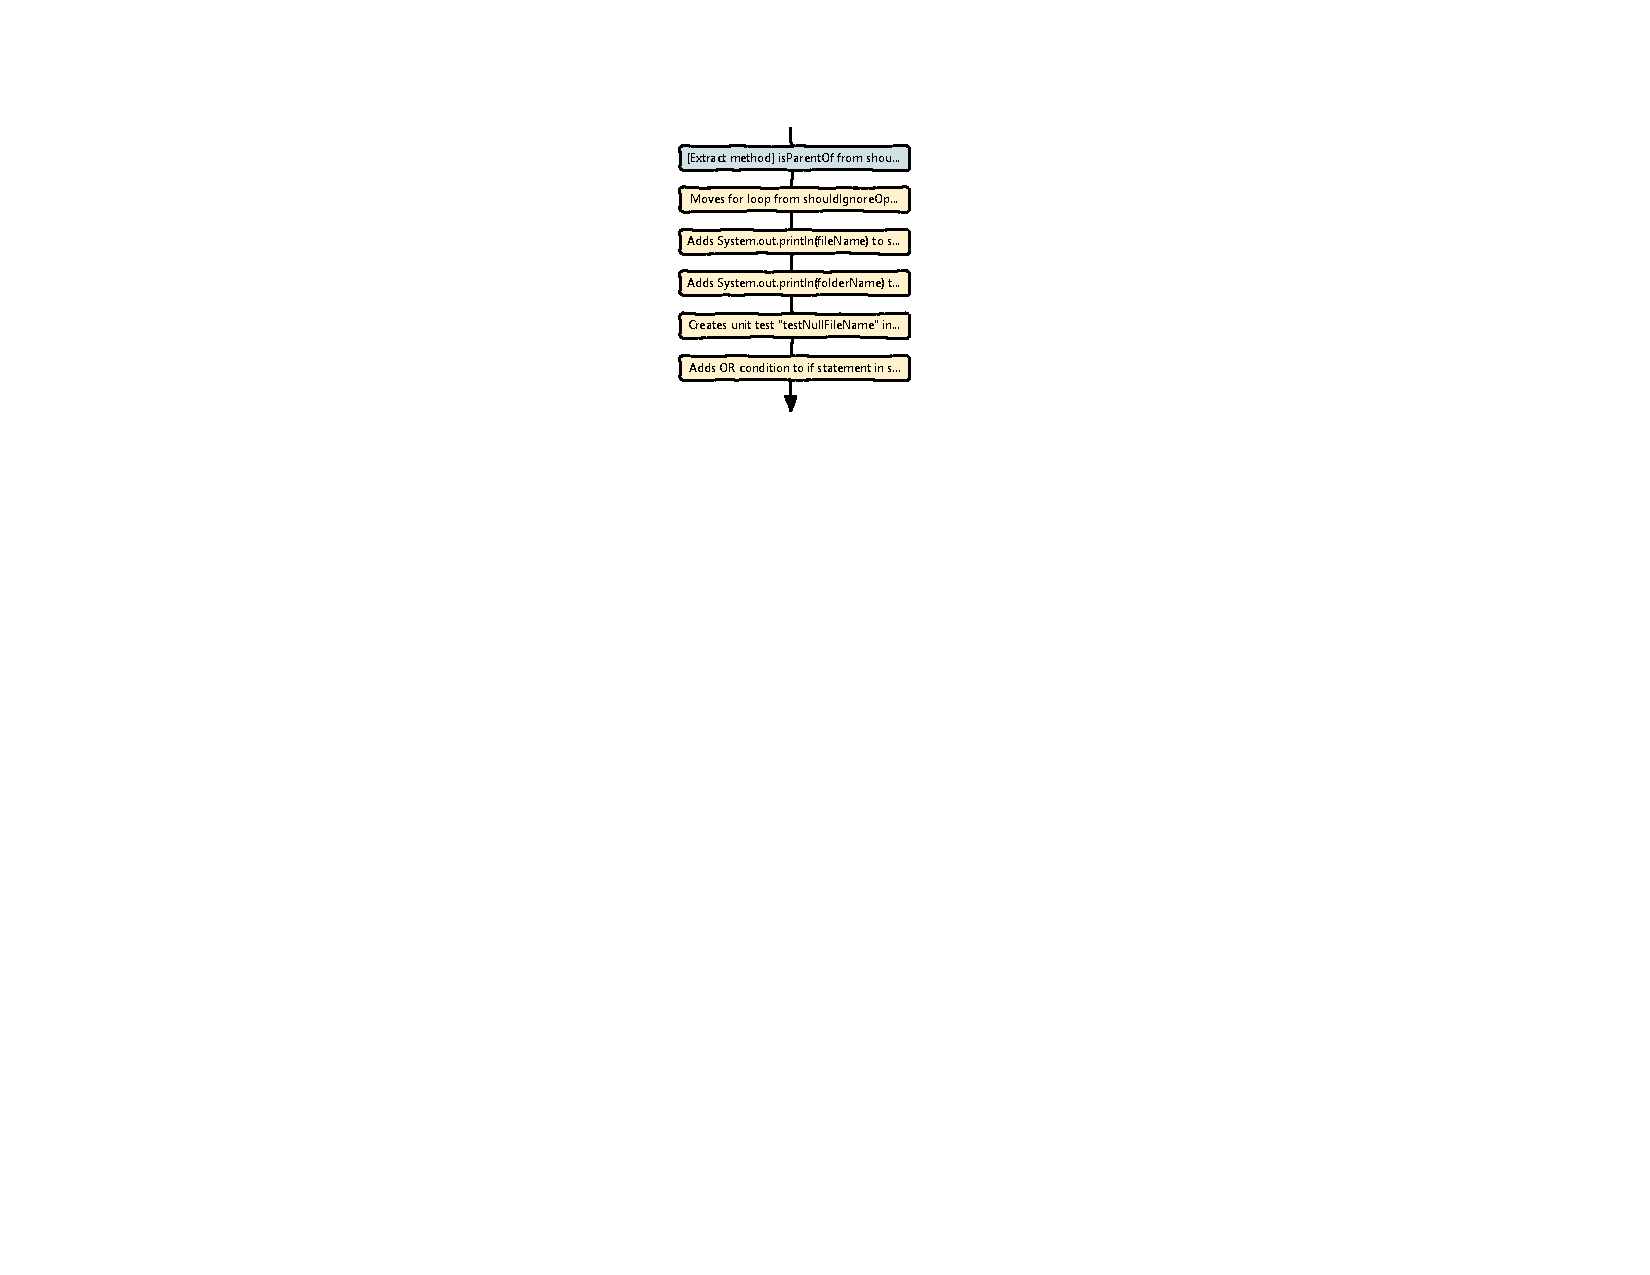
\includegraphics[height=2.1in]{bubblesAfterCheck}
\end{figure}
%The history looks something like: extract method isParentOf; moved for loop to isParentOf;
% adds debug statements;writes a test; adds null check

At this point his history is a bit of a mess, so Anthony decides to reorganize it.
First, he drags the creation of the unit test to the beginning where it is supposed to go, as per TDD standards.
\begin{figure}[h]
\centering
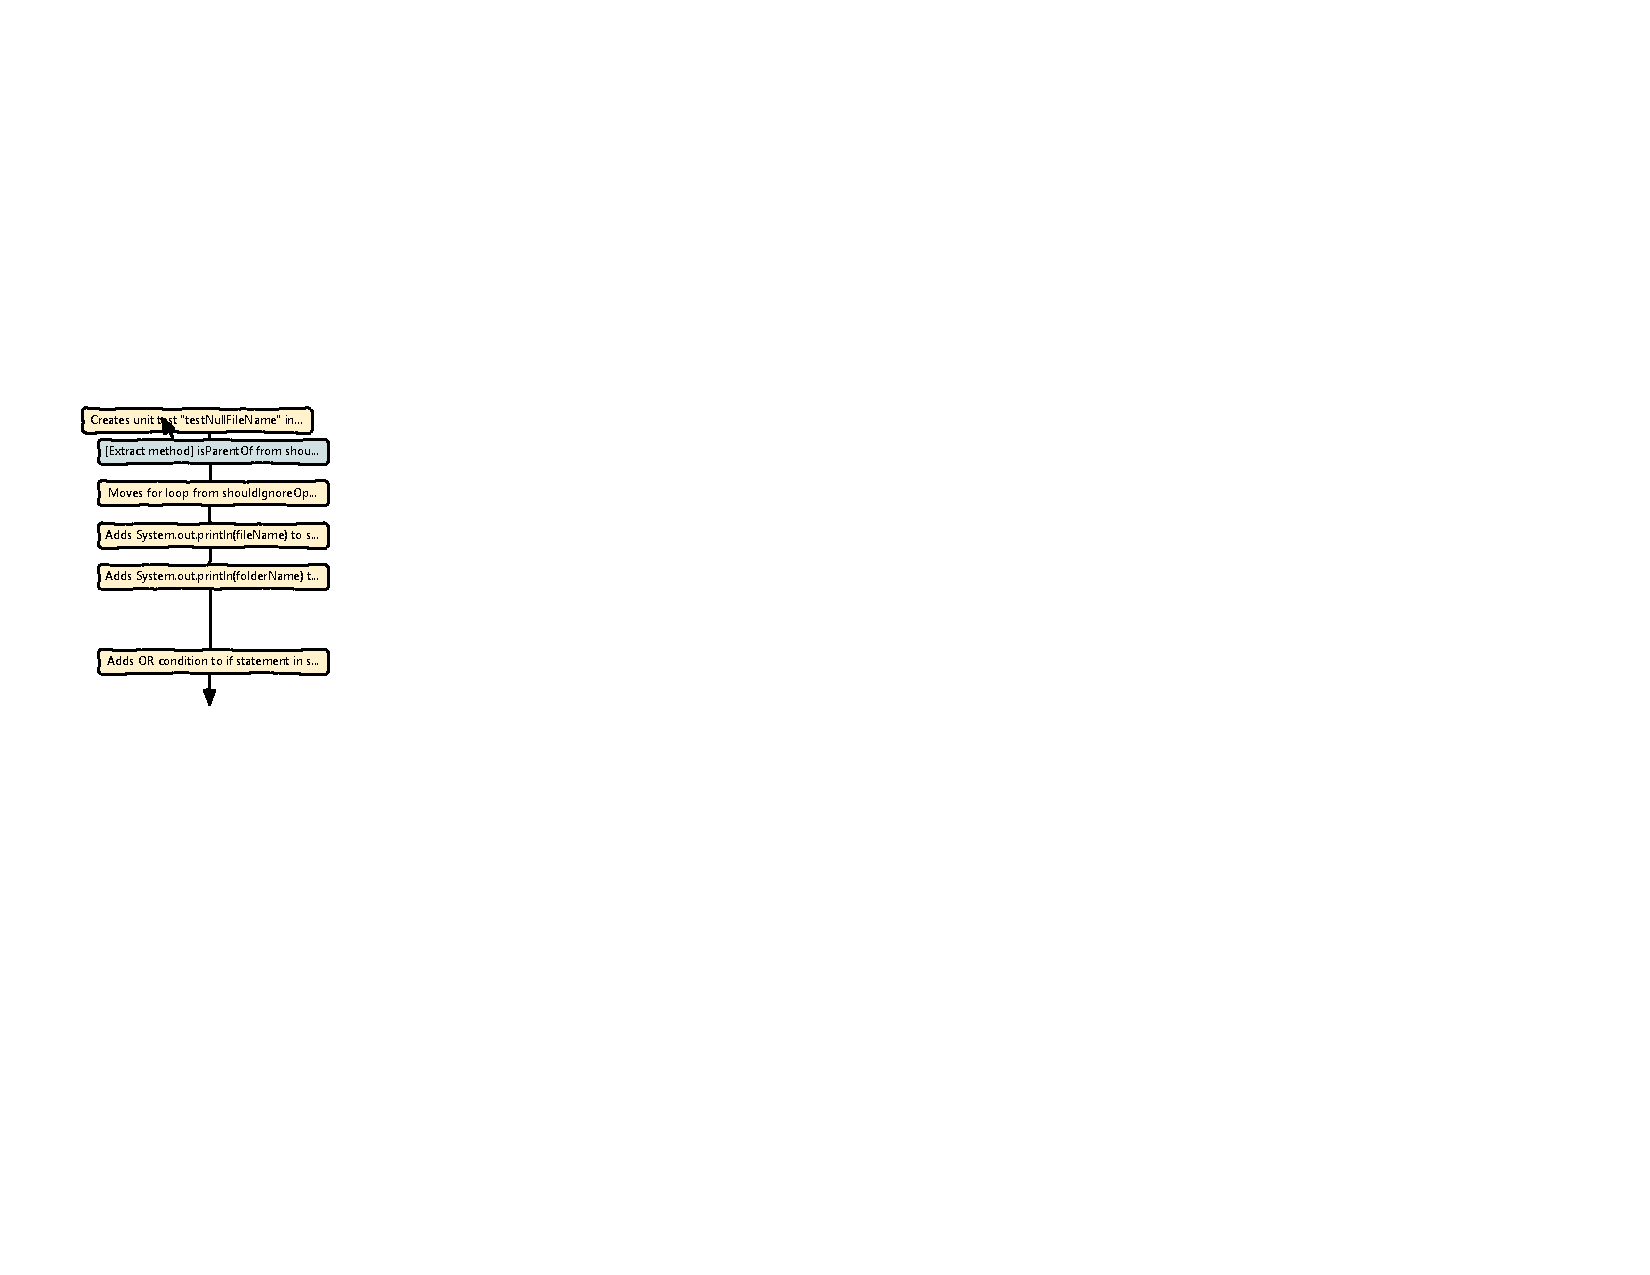
\includegraphics[height=2.1in]{reorder-during}
\end{figure}
%The history looks something like: writes a test; extract method isParentOf; moved for loop to isParentOf;
% adds debug statements; adds null check

Anthony doesn't want his debug statements in production, but he might still need them,
 so he breaks those out into his private branch with a simple drag gesture (Figure \ref{fig:private-branch}).
\begin{figure}[h]
\centering
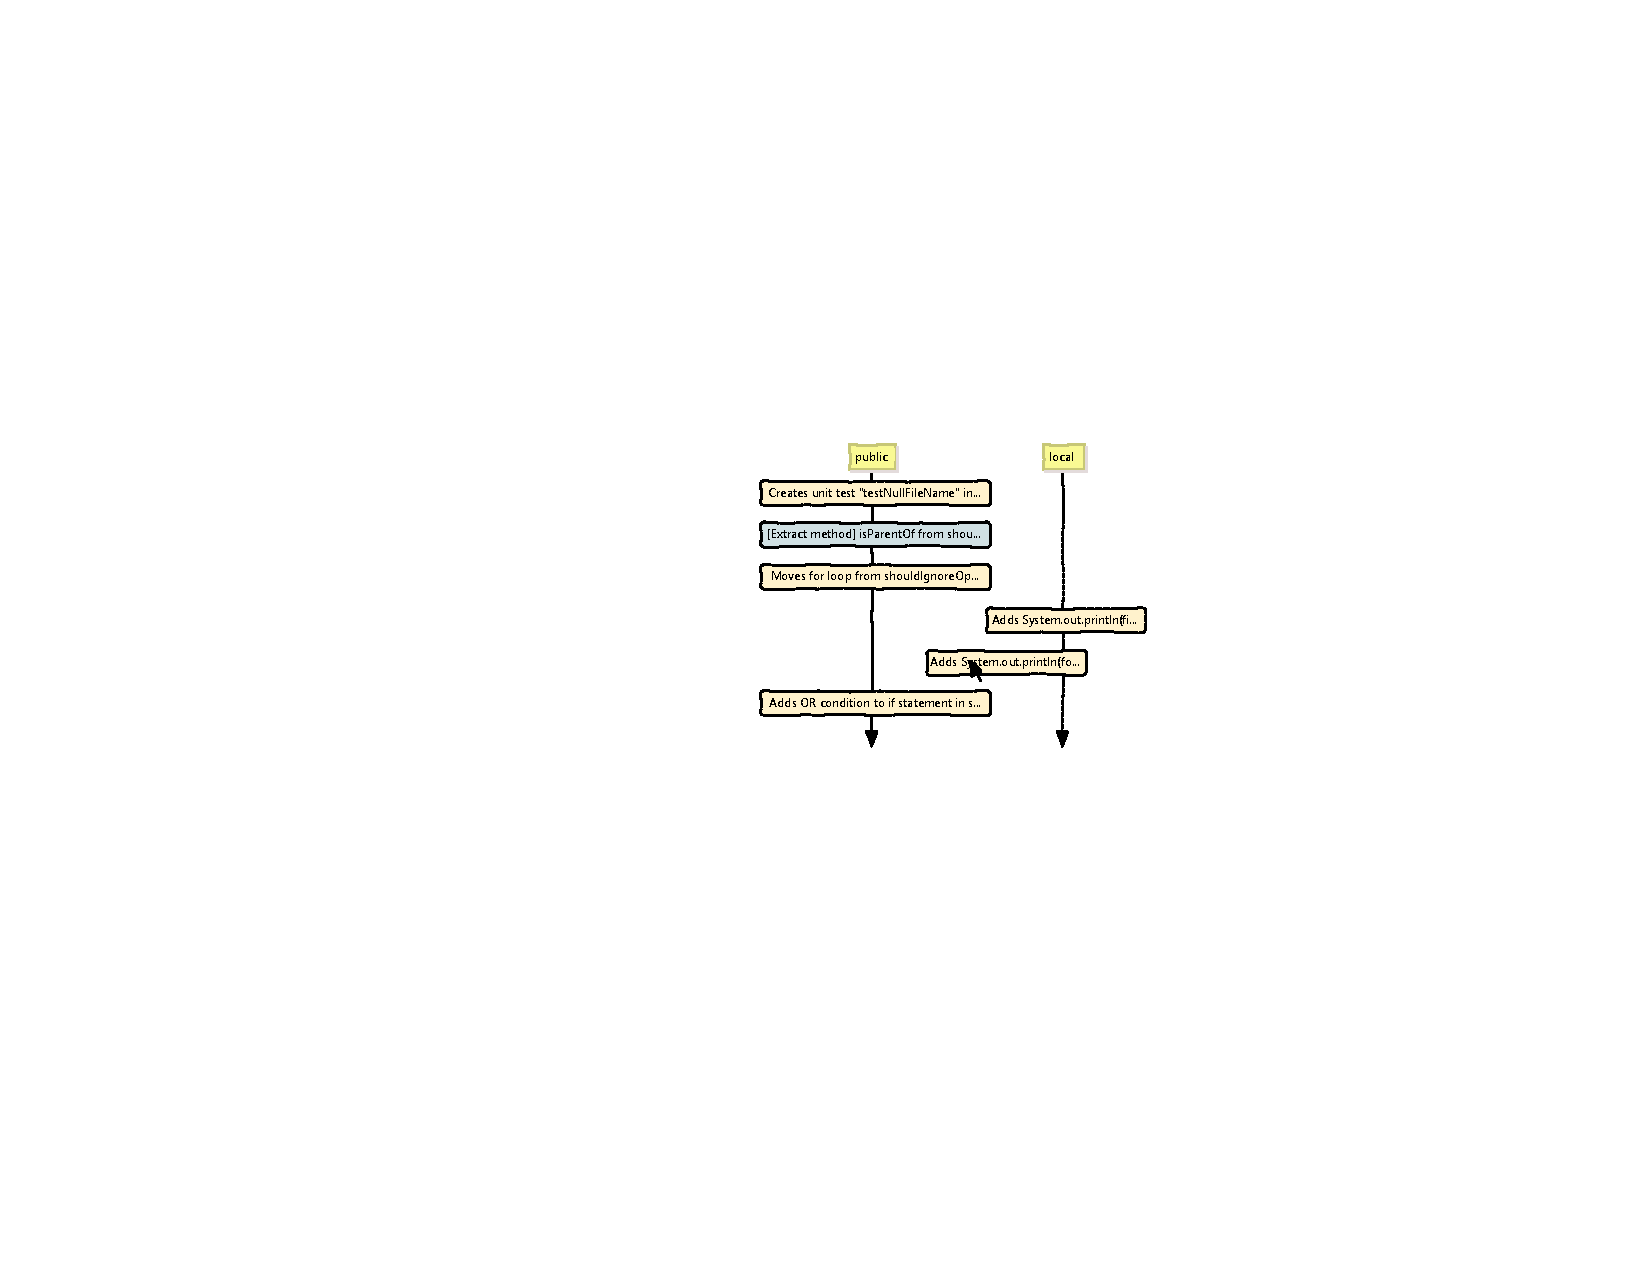
\includegraphics[height=2.1in]{breakout-during}
\caption{Breaking out changes into a private branch}
\label{fig:private-branch}
\end{figure}
%The history looks something like: writes a test; extract method isParentOf; moved for loop to isParentOf;
% adds null check   | adds debug statements; 

Finally, he combines the two refactoring bubbles into one because they were both needed to properly extract
the logic of isParentOf (Figure \ref{fig:merge}).
\begin{figure}[h]
\centering
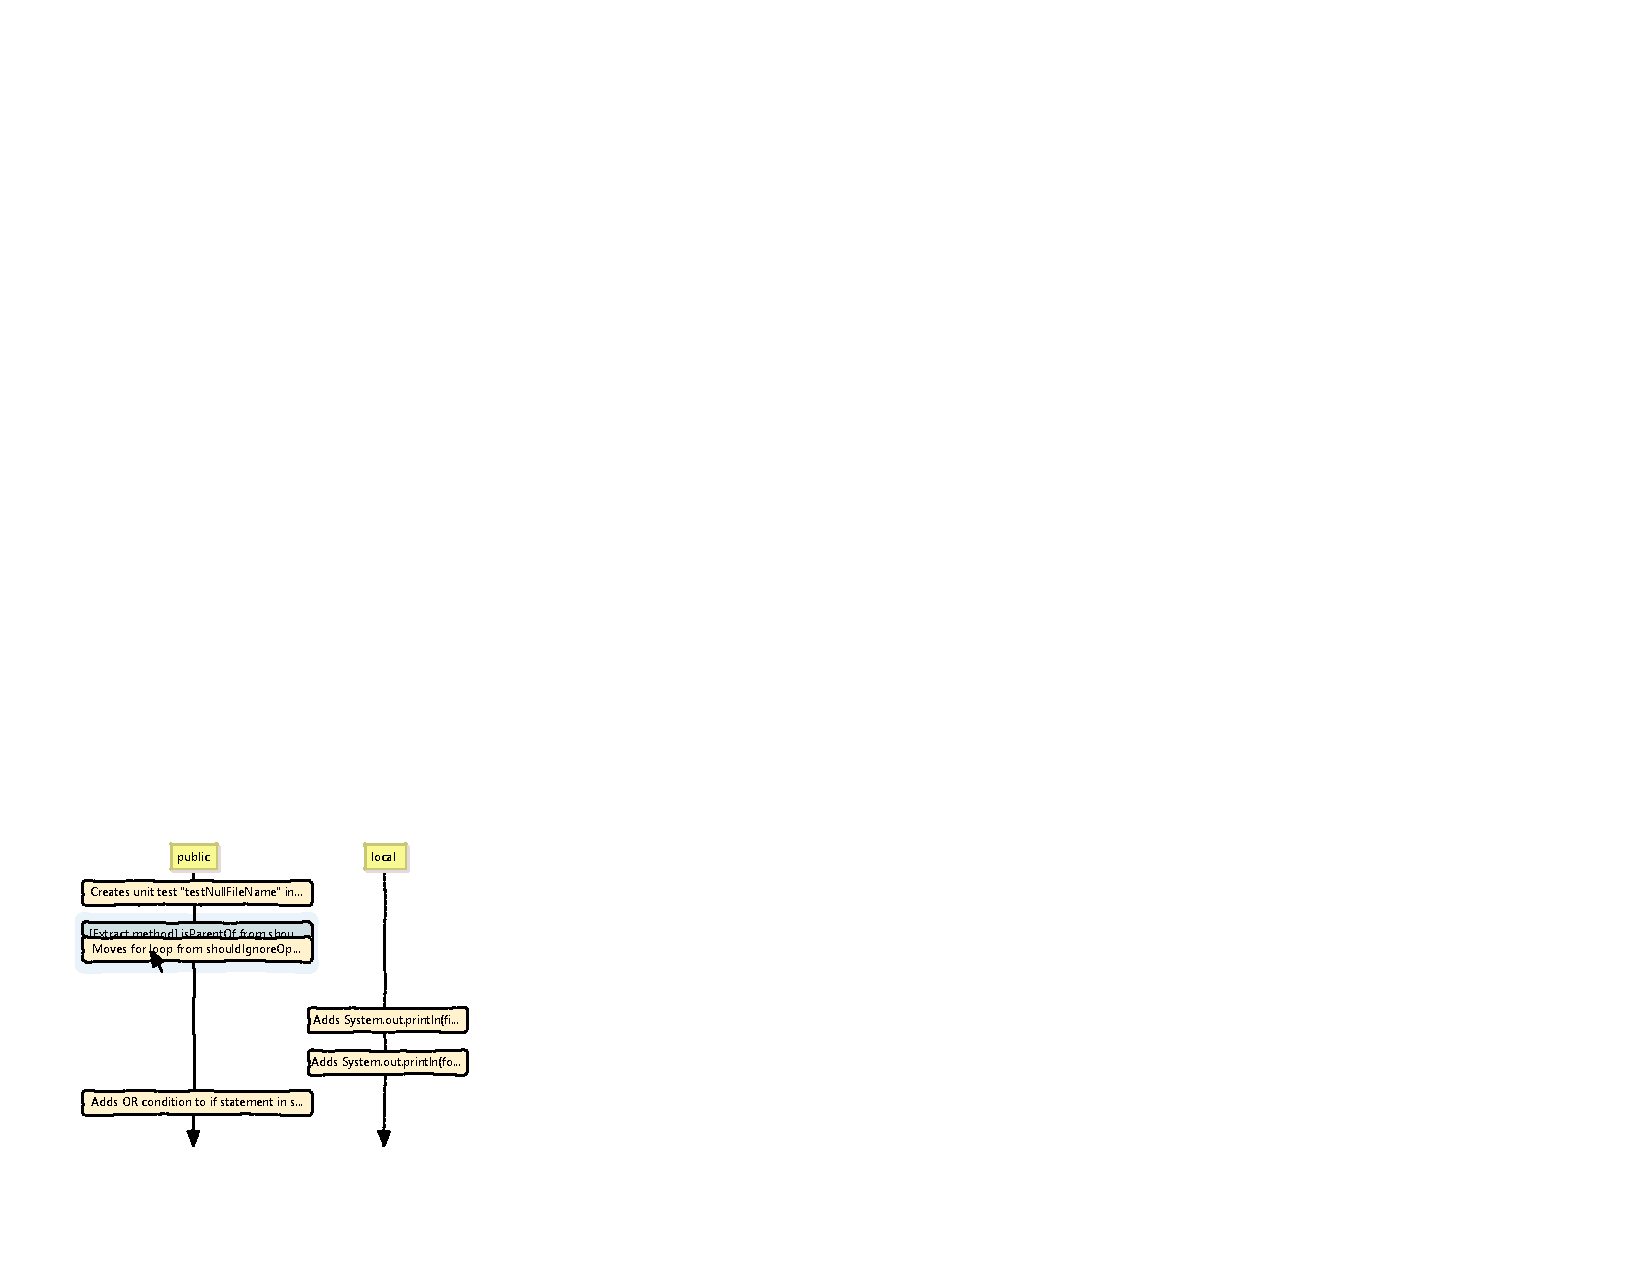
\includegraphics[height=2.1in]{merge-during}
\caption{Merging commit bubbles together using drag and drop}
\label{fig:merge}
\end{figure}
%The history looks something like: writes a test; (extract method isParentOf; moved for loop to isParentOf;)
% adds null check   | adds debug statements; 
He adjusts the commit messages of some bubbles, leaving his history as in Figure \ref{fig:fixed-history}, before pressing commit.

\begin{figure}[h]
\centering
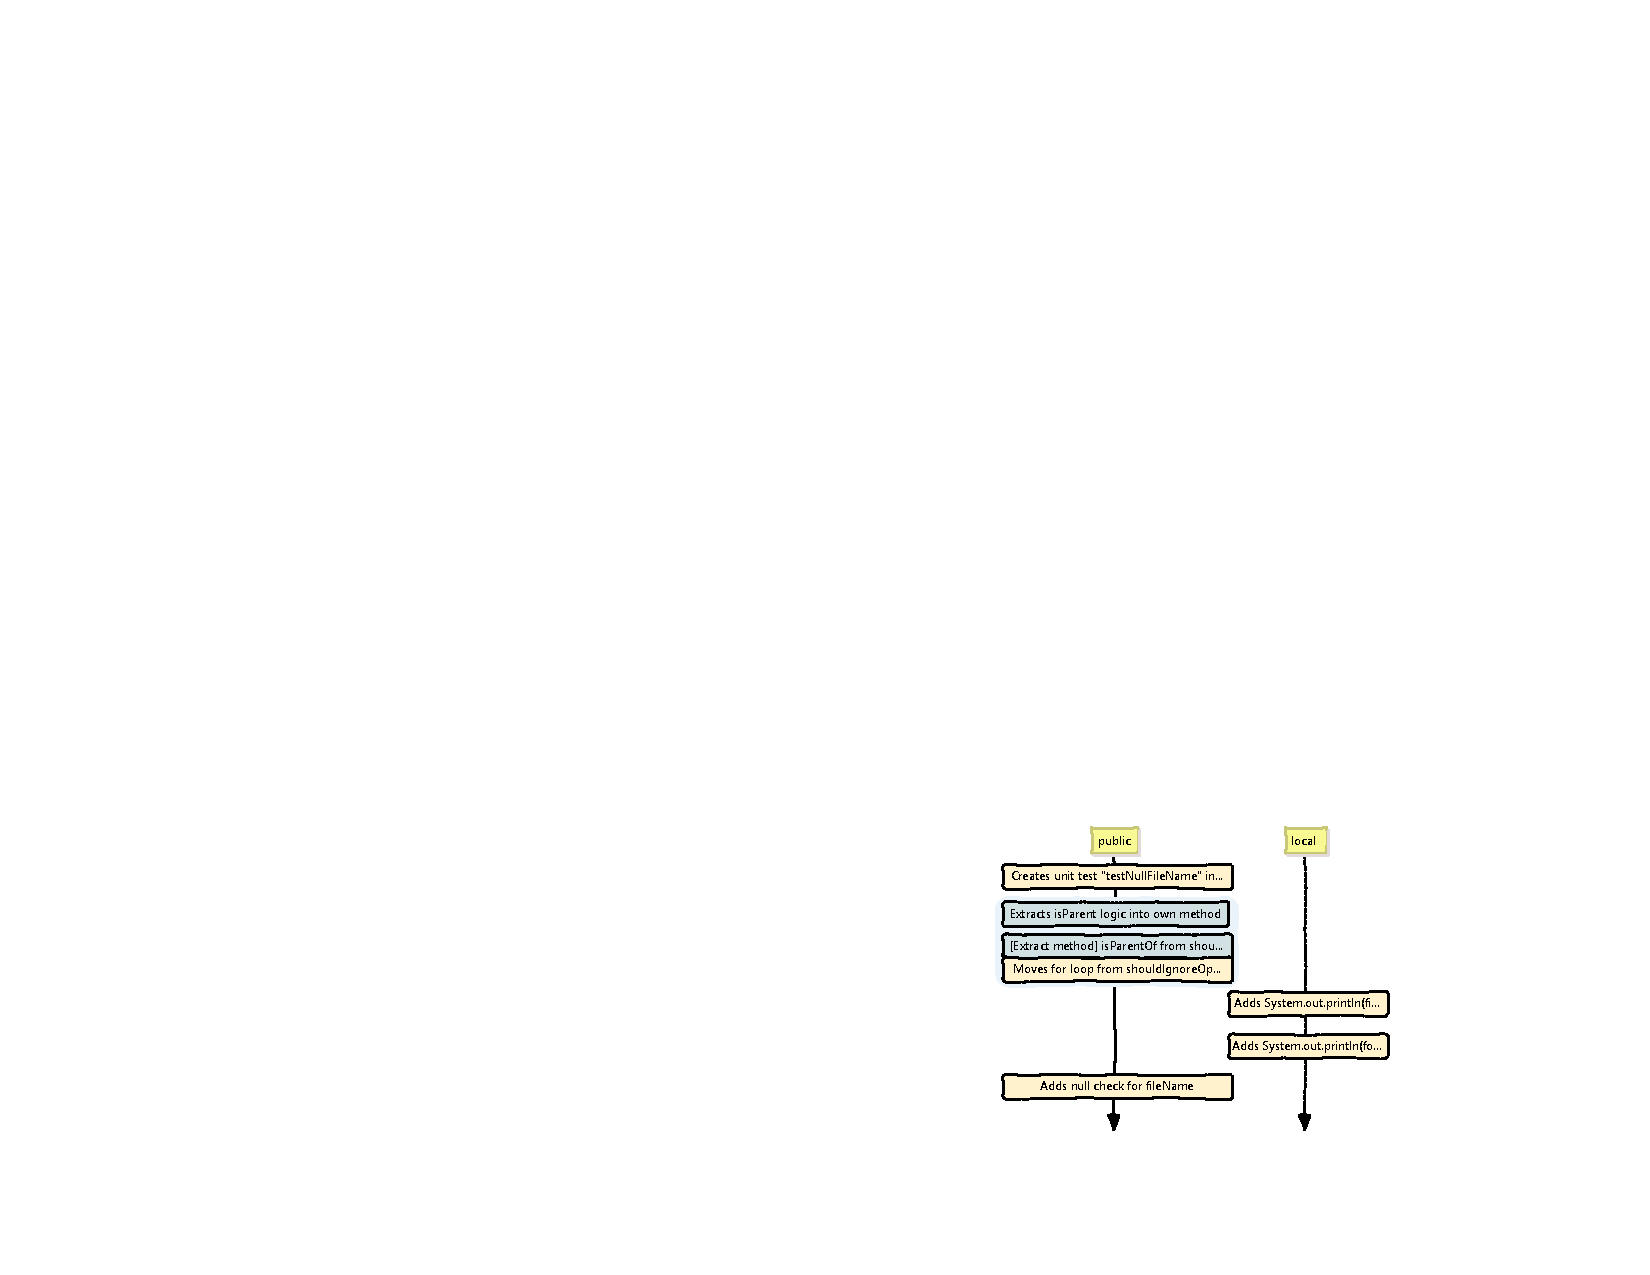
\includegraphics[height=2.1in]{fixed-history}
\caption{A revised history}
\label{fig:fixed-history}
\end{figure}
%The history looks something like: writes a test; (extract method isParentOf; moved for loop to isParentOf;) renamed to Extracted directory comparison to isParentOf
% adds null check   | adds debug statements; 

\section{Concrete Approach in Eclipse / Future Work}

eclipse plugin using http://www.eclipse.org/jgit/
ecj <-- ast
hooking into tools extension point to capture tool commands

%\section{Introduction}

%TODO are all of these things change tasks

%computers -- designed for productivity?

%ideas are ``integrated'', yet their tools are compartmentalized.

%version control systems.
%they are difficult because of compartmentalization vs. integration? (what is the cognitive theory for this?)

%examples of how they are different:

%evolution of flow in tools -> compartment to integrated

%proposed model -> integration as first class principle

%semantic resolution of the tool is different from the semantic resolution of the system

%screen capture of a mockup demonstrating this concept

\section{Related Work}

Bento box design~\cite{DeLine2010a}

refactoring edit history of source code~\cite{Hayashi2012}

why is this citation here? ``Messages written by programmers in version-control commit logs do not reliably indicate the presence of refactoring in the commit.''
floss versus root canal refactoring~\cite{Murphy-Hill2012c}

intro -- need more papers on comprehension during change maintenance tasks

techniques we can leverage?
inserts vertical whitespaces into code to improve readability~\cite{Wang2011}


talk about \emph{task context} model

stylecop
and today! https://gitcop.com/

% TODO make a workflow figure

maybe in introduction -- influence on tasks on programming behavior~\cite{Ying2011a}

also in introduction -- automatic segmentation of method code into
meaningful blocks to improve readability 

what's wrong with git. what are some problems and how do we know?~\cite{PerezDeRosso2013}

Wingerd and Seiwald
high-level best practices in software configuration management~\cite{Wingerd1998}

Coven combines features in a collaborative setting; probably closes in spirit to the type of thing that we're trying to accomplish.~\cite{Chu-Carroll2000}

crosscutting system artifacts
posits that many development tasks do have structure
launch point because it has a lot of good citations
task alignment?~\cite{Murphy2005}

some ncie fragments; mockup; structure on multidimensionality; again lock focused (hierarchical locking -- not a model needed anymore)
~\cite{Chu-Carroll2003}

infuse, ``experimental databases'', managing and coordinating source code changes; introduces term \emph{change propagation}~\cite{Perry1987}

inscape environment = ``Dividing the life-cycle into two distinct phases, development and maintenance, introduces a distinction that is not born out in practice.'' and ``tools that are knowledgeable about the process of system construction and evolution and work in symbiosis with the system builders and evolvers'' paper focuses a lot on formal specifications.~\cite{Perry1989}


% http://delivery.acm.org.prox.lib.ncsu.edu/10.1145/360000/355058/p88-chu-carroll.pdf?ip=152.14.136.96&id=355058&acc=ACTIVE%20SERVICE&key=6ABC8B4C00F6EE47.4D4702B0C3E38B35.4D4702B0C3E38B35.4D4702B0C3E38B35&CFID=596113106&CFTOKEN=10420211&__acm__=1415544717_ebea3078944a1cffe21be1875ddc99c8

% http://dl.acm.org.prox.lib.ncsu.edu/citation.cfm?id=1321647

% http://dl.acm.org.prox.lib.ncsu.edu/citation.cfm?id=605482

% http://ieeexplore.ieee.org.prox.lib.ncsu.edu/xpls/abs_all.jsp?arnumber=4509441&tag=1

TODO: model-driven engineering, is that the same? START HERE
 --> right model for person, not for computer
% http://www.emeraldinsight.com.prox.lib.ncsu.edu/doi/abs/10.1108/17440080910983556

% http://e-collection.library.ethz.ch/eserv.php?pid=eth:46754&dsID=eth-46754-01.pdf


\section{State of the world today}

auto-complete, flow breaking activity when writing commit messages because of lack of semantic information

run builds not on your repository but against last commit + change

light stacking system for changes

\section{Our approach}

git as a version control framework, not a version control system

- what are some other models of this
- legit? git-flow? superimpose model on API
http://www.eclipse.org/jgit/ <-- nice option for how to implement this

\footnote{\url{http://www.eclipse.org/jgit/}}

\section{Challenges}

-- implementation?
naive should be easy: capture tool usage directly  
hard: ghostfactor (changes without using tools) , but other people
 are addressing this: See 1, 2, 3 for better semantic support which our tools will be able to leverage
 
 - worst-case combinatorial, but look at techniques more pruning this space using common design patterns, heuristics (temporal heuristics) (accuracy of temporaral heuristics)
 
 -- minimal screen resolution, passive information, always-on vs. on-demand? CPU performance. ui management across multiple files. higher level operations --> rename, delete files.
 -- changes not in the IDE
 -- does everyone have to use the tool? what if they don't? do we lose all support?

 -- what if you need the low-level? you no longer have any mental model between the two
 
 http://importantshock.wordpress.com/2008/08/07/git-vs-mercurial/


\section{Conclusion}


need a nice concept for framing

\begin{figure}[!t]
\centering
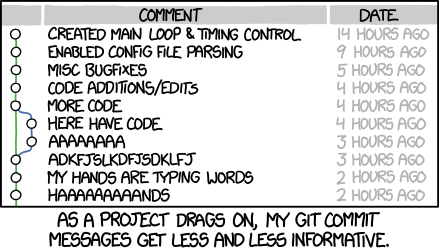
\includegraphics[width=\linewidth]{xkcd}
\caption{This is part of the problem.}
\label{fig:xkcd}
\end{figure}

% An example of a floating table. Note that, for IEEE style tables, the
% \caption command should come BEFORE the table. Table text will default to
% \footnotesize as IEEE normally uses this smaller font for tables.
% The \label must come after \caption as always.
%
%\begin{table}[!t]
%% increase table row spacing, adjust to taste
%\renewcommand{\arraystretch}{1.3}
% if using array.sty, it might be a good idea to tweak the value of
% \extrarowheight as needed to properly center the text within the cells
%\caption{An Example of a Table}
%\label{table_example}
%\centering
%% Some packages, such as MDW tools, offer better commands for making tables
%% than the plain LaTeX2e tabular which is used here.
%\begin{tabular}{|c||c|}
%\hline
%One & Two\\
%\hline
%Three & Four\\
%\hline
%\end{tabular}
%\end{table}


% Note that IEEE does not put floats in the very first column - or typically
% anywhere on the first page for that matter. Also, in-text middle ("here")
% positioning is not used. Most IEEE journals/conferences use top floats
% exclusively. Note that, LaTeX2e, unlike IEEE journals/conferences, places
% footnotes above bottom floats. This can be corrected via the \fnbelowfloat
% command of the stfloats package.

% use section* for acknowledgement
\section*{Acknowledgments}

I did this all by myself.


% trigger a \newpage just before the given reference
% number - used to balance the columns on the last page
% adjust value as needed - may need to be readjusted if
% the document is modified later
%\IEEEtriggeratref{8}
% The "triggered" command can be changed if desired:
%\IEEEtriggercmd{\enlargethispage{-5in}}

% references section

% can use a bibliography generated by BibTeX as a .bbl file
% BibTeX documentation can be easily obtained at:
% http://www.ctan.org/tex-archive/biblio/bibtex/contrib/doc/
% The IEEEtran BibTeX style support page is at:
% http://www.michaelshell.org/tex/ieeetran/bibtex/
\bibliographystyle{IEEEtran}
% argument is your BibTeX string definitions and bibliography database(s)
\bibliography{library}



% that's all folks
\end{document}


